% vim: set spell spelllang=en tw=100 et sw=4 sts=4 :

\documentclass[a1paper]{tikzposter}

\usepackage{microtype}
\usepackage{tikz}
\usepackage{amssymb}
\usepackage{amsmath}
\usepackage{pifont}
\usepackage{qrcode}

\usepackage{lmodern}
\renewcommand*\familydefault{\sfdefault}
\usepackage[T1]{fontenc}

\usetikzlibrary{positioning, backgrounds, scopes, calc, fit, graphs, graphs.standard, shapes.geometric,
shapes.multipart, arrows, arrows.meta, decorations, decorations.markings}

\title{Auditable Algorithms for Constraint Optimisation}
\author{Arthur Gontier, Ciaran McCreesh, and
Matthew McIlree}
\institute{University of Glasgow, Glasgow, Scotland}

\settitle{
    \begin{tikzpicture}
        \node (T) [inner xsep=0pt, inner ysep=-50pt] {\begin{minipage}{\linewidth}
                \color{titlefgcolor}
                {\bfseries \huge \@title \par}
                \vspace*{0.6em}
                {\large {\bfseries \@author} \\[0.1em] \@institute}
                \vspace*{0.6em}

                {\small With numerous co-conspirators, including Jeremias Berg (University of
                Helsinki), Bart
                Bogaerts and Dieter Vandesande (VU Brussels), Emir \\ Demirovi\'c and Konstantin Sidorov (TU Delft), Stephan
                Gocht, Jakob Nordstr{\"o}m and Andy Oertel (Lund University and University of
                Copenhagen), \\ Magnus O. Myreen (Chalmers University), and
                Yong Kiam Tan (I$^2$R, A$\star$STAR)}
        \end{minipage}};

        \coordinate (logopos) at (T.east);

        \node at (logopos) [anchor=center, inner sep=0pt, xshift=0cm, yshift=2.3cm,
        xshift=-5.5cm] {
            
\includegraphics[keepaspectratio=true,height=3.0cm]{../../images/UoG_keyline.pdf}
        };

        \node at (logopos) [anchor=center, inner sep=0pt, xshift=0cm, yshift=-2.3cm,
        xshift=-5.5cm] {
            
\includegraphics[keepaspectratio=true,height=3.0cm]{../../images/RAEngWhite.pdf}
        };
    \end{tikzpicture}
}

% University of Glasgow standard colours
\definecolor{uofguniversityblue}{rgb}{0, 0.219608, 0.396078}

\definecolor{uofgheather}{rgb}{0.356863, 0.32549, 0.490196}
\definecolor{uofgaquamarine}{rgb}{0.603922, 0.72549, 0.678431}
\definecolor{uofgslate}{rgb}{0.309804, 0.34902, 0.380392}
\definecolor{uofgrose}{rgb}{0.823529, 0.470588, 0.709804}
\definecolor{uofgmocha}{rgb}{0.709804, 0.564706, 0.47451}

\definecolor{uofglawn}{rgb}{0.517647, 0.741176, 0}
\definecolor{uofgleaf}{rgb}{0, 0.517647, 0.239216}
\definecolor{uofgcobalt}{rgb}{0, 0.615686, 0.92549}
\definecolor{uofgturquoise}{rgb}{0, 0.709804, 0.819608}
\definecolor{uofgsunshine}{rgb}{1.0, 0.862745, 0.211765}
\definecolor{uofgpumpkin}{rgb}{1.0, 0.72549, 0.282353}
\definecolor{uofgthistle}{rgb}{0.584314, 0.070588, 0.447059}
\definecolor{uofgpillarbox}{rgb}{0.701961, 0.047059, 0}
\definecolor{uofglavendar}{rgb}{0.356863, 0.301961, 0.580392}

\definecolor{uofgsandstone}{rgb}{0.321569, 0.278431, 0.231373}
\definecolor{uofgforest}{rgb}{0, 0.317647, 0.2}
\definecolor{uofgburgundy}{rgb}{0.490196, 0.133333, 0.223529}
\definecolor{uofgrust}{rgb}{0.603922, 0.227451, 0.023529}

\definecolorstyle{UofG}{
}{
    % Background Colors
    \colorlet{backgroundcolor}{uofgsandstone!40!white}
    \colorlet{framecolor}{black}
    % Title Colors
    \colorlet{titlefgcolor}{white}
    \colorlet{titlebgcolor}{uofguniversityblue}
    % Block Colors
    \colorlet{blocktitlebgcolor}{white}
    \colorlet{blocktitlefgcolor}{uofguniversityblue}
    \colorlet{blockbodybgcolor}{white}
    \colorlet{blockbodyfgcolor}{black}
    % Innerblock Colors
    \colorlet{innerblocktitlebgcolor}{uofguniversityblue}
    \colorlet{innerblocktitlefgcolor}{black}
    \colorlet{innerblockbodybgcolor}{uofgsandstone}
    \colorlet{innerblockbodyfgcolor}{black}
    % Note colors
    \colorlet{notefgcolor}{black}
    \colorlet{notebgcolor}{uofgrust}
    \colorlet{noteframecolor}{red}
}

\usetheme{Autumn}
\usecolorstyle{UofG}

\tikzposterlatexaffectionproofoff

\useblockstyle[bodyverticalshift=-1cm, roundedcorners=1]{Default}

\renewcommand{\Huge}{\fontsize{77.2}{96}\selectfont}

% Styles for drawings

\tikzset{edge/.style={line width=3pt, color=uofgsandstone}}
\tikzset{ledge/.style={line width=3pt, color=uofgsandstone!40!white}}

\setlength\intextsep{0pt}

\newcommand{\truck}[1]{
    \begin{tikzpicture}[scale=1.5, inner sep=0pt, outer sep=0pt]
        \path[fill=uofgsandstone] (0.9525, -0.7144).. controls (0.9525, -0.7728) and (0.9051, -0.8202) .. (0.8467, -0.8202) -- (0.1058, -0.8202).. controls (0.0474, -0.8202) and (0.0, -0.7728) .. (0.0, -0.7144) -- (0.0, -0.635).. controls (0.0, -0.5766) and (0.0474, -0.5292) .. (0.1058, -0.5292) -- (0.8467, -0.5292).. controls (0.9051, -0.5292) and (0.9525, -0.5766) .. (0.9525, -0.635) -- (0.9525, -0.7144) -- cycle;
        \path[fill=uofgsandstone!60!white] (0.5027, -0.344) -- (0.4768, -0.3175) -- (0.1891, -0.3175).. controls (0.1058, -0.3175) and (0.0794, -0.3704) .. (0.0794, -0.3704) -- (0.0, -0.5281) -- (0.0, -0.6615) -- (0.5027, -0.6615) -- (0.5027, -0.344) -- cycle;
        \path[fill=uofgsandstone!40!white] (0.2381, -0.5292) -- (0.0529, -0.5292) -- (0.1058, -0.4233) -- (0.2381, -0.3704) -- (0.2381, -0.5292) -- cycle;
        \path[fill=uofgsandstone!40!white] (0.2381, -0.8202) circle (0.1058cm);
        \path[fill=black] (0.2381, -0.8202) circle (0.0529cm);
        \path[fill=uofgsandstone!40!white] (0.7144, -0.8202) circle (0.1058cm);
        \path[fill=black] (0.7144, -0.8202) circle (0.0529cm);
        \path[fill=#1] (0.8467, -0.2117) -- (0.4498, -0.2117).. controls (0.3913, -0.2117) and (0.344, -0.2591) .. (0.344, -0.3175) -- (0.344, -0.6615) -- (0.9525, -0.6615) -- (0.9525, -0.3175).. controls (0.9525, -0.2591) and (0.9051, -0.2117) .. (0.8467, -0.2117) -- cycle;
    \end{tikzpicture}
}

\newcommand{\parcel}{
\includegraphics[width=1.2em]{parcel.pdf}\,}
\newcommand{\trashpanda}{
\includegraphics[width=1.2em]{trashpanda.pdf}\,}
\newcommand{\bed}{
\includegraphics[width=1.2em]{bed.pdf}\,}
\newcommand{\chair}{
\includegraphics[width=1.2em]{chair.pdf}\,}
\newcommand{\tree}{
\includegraphics[width=1.2em]{tree.pdf}\,}
\newcommand{\present}{
\includegraphics[width=1.2em]{present.pdf}\,}
\newcommand{\laptop}{
\includegraphics[width=1.2em]{laptop.pdf}\,}
\newcommand{\drivera}{
\includegraphics[width=1.2em]{driver1.pdf}\,}
\newcommand{\driverb}{
\includegraphics[width=1.2em]{driver2.pdf}\,}

\begin{document}
\maketitle

{
    \colorlet{blockbodybgcolor}{uofgcobalt}
    \colorlet{blocktitlebgcolor}{uofgcobalt}
    \block[bodyverticalshift=0cm, bodyinnersep=3mm]{}{
        \centering\begin{minipage}{0.90\textwidth}
            \textbf{Why should you believe an algorithm is giving you the right answer?}
            Increasingly complex ``intelligent'' algorithms are being deployed in ways that
            directly affect your life and livelihood, and often no-one knows whether these algorithms are
            designed and implemented correctly. We can fix this by
            \textbf{trusting solutions, not solvers}: by making solving algorithms show their
            work in a verifiable way, we can \textbf{independently audit solutions} for correctness
            and optimality. This does not mean an algorithm is free from bugs or maliciousness, but
            it does mean that if it ever gives a wrong answer, it can always be detected.
        \end{minipage}
    }
}

\begin{columns}
\column{0.45}
\block{Constraint Programming}{
    We express a problem in terms of \textbf{variables} which have a \textbf{domain} of possible
    values, together with \textbf{constraints} and an \textbf{objective function}. The constraints
    can be of different, expressive kinds, such as ``all different'', ``forms a tour'',
    and ``can be packed inside a van with these dimensions''.
    A \textcolor{uofgrust}{solver} works out the best answer.

    \bigskip
    \bigskip

    \begin{center}
    \begin{minipage}{10cm}
        \centering
        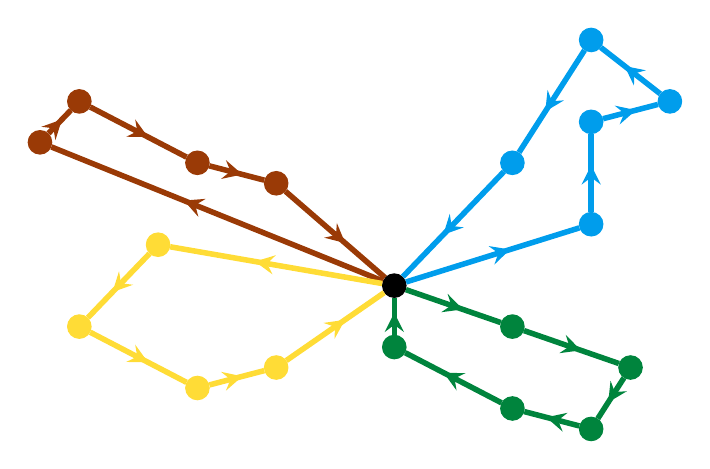
\begin{tikzpicture}
        \begin{scope}[yscale=2.6, xscale=5.0]
        \node (depot) [inner sep=3pt, draw, fill, circle] at (0,0) {};

        \node (RC1) [inner sep=3pt, draw, fill, circle, color=uofgcobalt] at (0.5,0.3) {};
        \node (RC2) [inner sep=3pt, draw, fill, circle, color=uofgcobalt] at (0.5,0.8) {};
        \node (RC3) [inner sep=3pt, draw, fill, circle, color=uofgcobalt] at (0.7,0.9) {};
        \node (RC4) [inner sep=3pt, draw, fill, circle, color=uofgcobalt] at (0.5,1.2) {};
        \node (RC5) [inner sep=3pt, draw, fill, circle, color=uofgcobalt] at (0.3,0.6) {};

        \begin{scope}[decoration={markings, mark=at position 0.6 with {\arrow{stealth}}}]
            \draw [postaction={decorate}, line width=2pt, color=uofgcobalt] (depot) -- (RC1);
            \draw [postaction={decorate}, line width=2pt, color=uofgcobalt] (RC1)   -- (RC2);
            \draw [postaction={decorate}, line width=2pt, color=uofgcobalt] (RC2)   -- (RC3);
            \draw [postaction={decorate}, line width=2pt, color=uofgcobalt] (RC3)   -- (RC4);
            \draw [postaction={decorate}, line width=2pt, color=uofgcobalt] (RC4)   -- (RC5);
            \draw [postaction={decorate}, line width=2pt, color=uofgcobalt] (RC5)   -- (depot);
        \end{scope}

        \node (RR1) [inner sep=3pt, draw, fill, circle, color=uofgrust] at (-0.9,0.7) {};
        \node (RR2) [inner sep=3pt, draw, fill, circle, color=uofgrust] at (-0.8,0.9) {};
        \node (RR3) [inner sep=3pt, draw, fill, circle, color=uofgrust] at (-0.5,0.6) {};
        \node (RR4) [inner sep=3pt, draw, fill, circle, color=uofgrust] at (-0.3,0.5) {};

        \begin{scope}[decoration={markings, mark=at position 0.6 with {\arrow{stealth}}}]
            \draw [postaction={decorate}, line width=2pt, color=uofgrust] (depot) -- (RR1);
            \draw [postaction={decorate}, line width=2pt, color=uofgrust] (RR1)   -- (RR2);
            \draw [postaction={decorate}, line width=2pt, color=uofgrust] (RR2)   -- (RR3);
            \draw [postaction={decorate}, line width=2pt, color=uofgrust] (RR3)   -- (RR4);
            \draw [postaction={decorate}, line width=2pt, color=uofgrust] (RR4)   -- (depot);
        \end{scope}

        \node (RS1) [inner sep=3pt, draw, fill, circle, color=uofgsunshine] at (-0.6,0.2) {};
        \node (RS2) [inner sep=3pt, draw, fill, circle, color=uofgsunshine] at (-0.8,-0.2) {};
        \node (RS3) [inner sep=3pt, draw, fill, circle, color=uofgsunshine] at (-0.5,-0.5) {};
        \node (RS4) [inner sep=3pt, draw, fill, circle, color=uofgsunshine] at (-0.3,-0.4) {};

        \begin{scope}[decoration={markings, mark=at position 0.6 with {\arrow{stealth}}}]
            \draw [postaction={decorate}, line width=2pt, color=uofgsunshine] (depot) -- (RS1);
            \draw [postaction={decorate}, line width=2pt, color=uofgsunshine] (RS1)   -- (RS2);
            \draw [postaction={decorate}, line width=2pt, color=uofgsunshine] (RS2)   -- (RS3);
            \draw [postaction={decorate}, line width=2pt, color=uofgsunshine] (RS3)   -- (RS4);
            \draw [postaction={decorate}, line width=2pt, color=uofgsunshine] (RS4)   -- (depot);
        \end{scope}

        \node (RL1) [inner sep=3pt, draw, fill, circle, color=uofgleaf] at (0.3,-0.2) {};
        \node (RL2) [inner sep=3pt, draw, fill, circle, color=uofgleaf] at (0.6,-0.4) {};
        \node (RL3) [inner sep=3pt, draw, fill, circle, color=uofgleaf] at (0.5,-0.7) {};
        \node (RL4) [inner sep=3pt, draw, fill, circle, color=uofgleaf] at (0.3,-0.6) {};
        \node (RL5) [inner sep=3pt, draw, fill, circle, color=uofgleaf] at (0,-0.3) {};

        \begin{scope}[decoration={markings, mark=at position 0.6 with {\arrow{stealth}}}]
            \draw [postaction={decorate}, line width=2pt, color=uofgleaf] (depot) -- (RL1);
            \draw [postaction={decorate}, line width=2pt, color=uofgleaf] (RL1)   -- (RL2);
            \draw [postaction={decorate}, line width=2pt, color=uofgleaf] (RL2)   -- (RL3);
            \draw [postaction={decorate}, line width=2pt, color=uofgleaf] (RL3)   -- (RL4);
            \draw [postaction={decorate}, line width=2pt, color=uofgleaf] (RL4)   -- (RL5);
            \draw [postaction={decorate}, line width=2pt, color=uofgleaf] (RL5)   -- (depot);
        \end{scope}
        \end{scope}
    \end{tikzpicture}
\end{minipage}\begin{minipage}{12cm}
    \truck{uofgrust} \drivera\driverb\raisebox{3mm}{:} \bed\parcel\chair\parcel

    \truck{uofgcobalt} \driverb\drivera\raisebox{3mm}{:}
    \chair\trashpanda\parcel\parcel\present

    \truck{uofgsunshine} \driverb\driverb\raisebox{3mm}{:} \tree\parcel\chair\present

    \truck{uofgleaf} \drivera\phantom{\drivera}\raisebox{3mm}{:}
    \parcel\parcel\laptop\parcel\parcel
\end{minipage}
\end{center}
}
\column{0.55}
\block{Proof Logging}{
    \begin{center}
    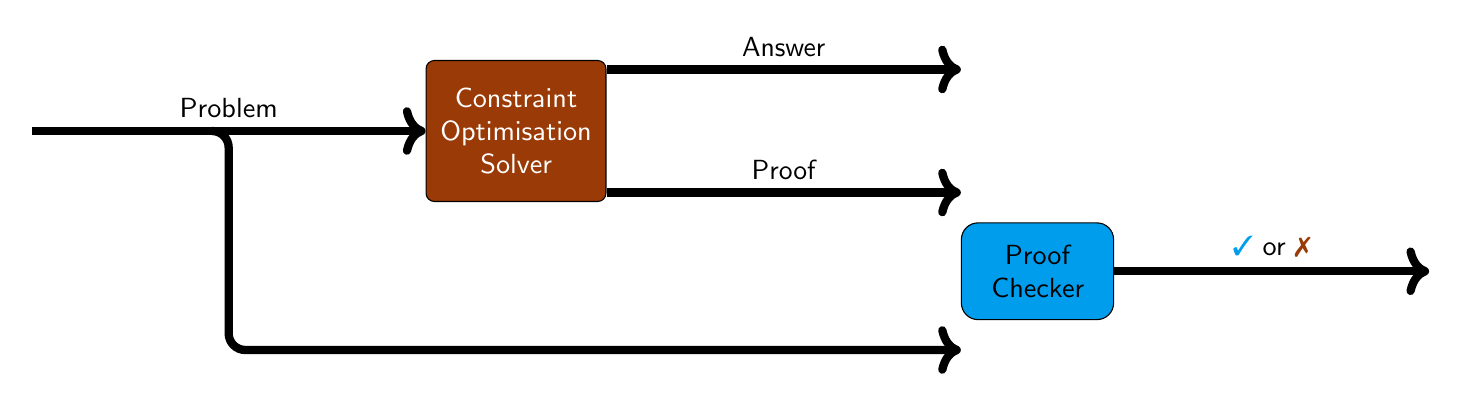
\begin{tikzpicture}
        \node (solver) [text centered, text width=5.5em, inner xsep=0.5em, inner ysep=1em, draw, rounded
        corners=3pt, fill=uofgrust, text=white] { Constraint Optimisation Solver };

        \node (checker) [ right=4.5cm of solver.south east, anchor=south west, inner
        xsep=0.25em, draw, rounded corners=6pt, text width=4.5em, text centered,
        fill=uofgcobalt, inner xsep=0.5em, inner ysep=0.8em, yshift=-1.5cm] { Proof Checker };

        \coordinate [left=5.0cm of solver.west] (input);
        \draw [->, line width=3pt] (input) -- (solver.west) coordinate [midway] (inputmid) node [above,
        midway, text width=5em, text centered] { Problem };

        \coordinate [right=4.0cm of checker.east] (ding);
        \draw [->, line width=3pt] (checker.east) -- (ding) node [above,
        midway, text width=5em, text centered] { \textcolor{uofgcobalt}{\ding{51}} or
        \textcolor{uofgrust}{\ding{55}} };

        \coordinate (proofin) at ($(checker.west)+(0cm,1cm)$);
        \draw [->, line width=3pt] (solver.east|-proofin) -- (proofin) node [above,
        midway, text centered] { Proof };

        \coordinate (resultout) at ($(solver.north east)+(solver.south east)-(solver.east|-proofin)$);
        \draw [->, line width=3pt] (resultout) -- (resultout-|proofin) node [above,
        midway, text centered] { Answer };

        \coordinate (checkerproblemin) at ($(checker.west)+(0cm,-1cm)$);
        \draw [->, line width=3pt, rounded corners=6pt] ($(inputmid)+(-0.2,0)$) -- (inputmid) -- (inputmid |-
        checkerproblemin) -- (checkerproblemin);

    \end{tikzpicture}\end{center}

    \smallskip

    As well as a solution, we make the \textcolor{uofgrust}{solver} output a machine-readable proof. We only consider the
    solution to be correct if a \textcolor{uofgcobalt}{proof checker} accepts the proof. This proof
    can be stored, and independently audited. The proof checker is very
    simple, so it is easier to trust.
}
\end{columns}

{
    \colorlet{blockbodybgcolor}{uofgrust}
    \colorlet{blockbodyfgcolor}{white}
    \colorlet{blocktitlebgcolor}{uofgrust}
    \block[bodyverticalshift=0cm, bodyinnersep=6mm]{}{
        \centering\begin{minipage}{0.90\textwidth}
\Huge \centering Algorithms contain bugs. Don't trust them!
        \end{minipage}
    }
}

\block{From a Human-Readable Problem Description to a Trusted Solution}{
    \begin{center}
    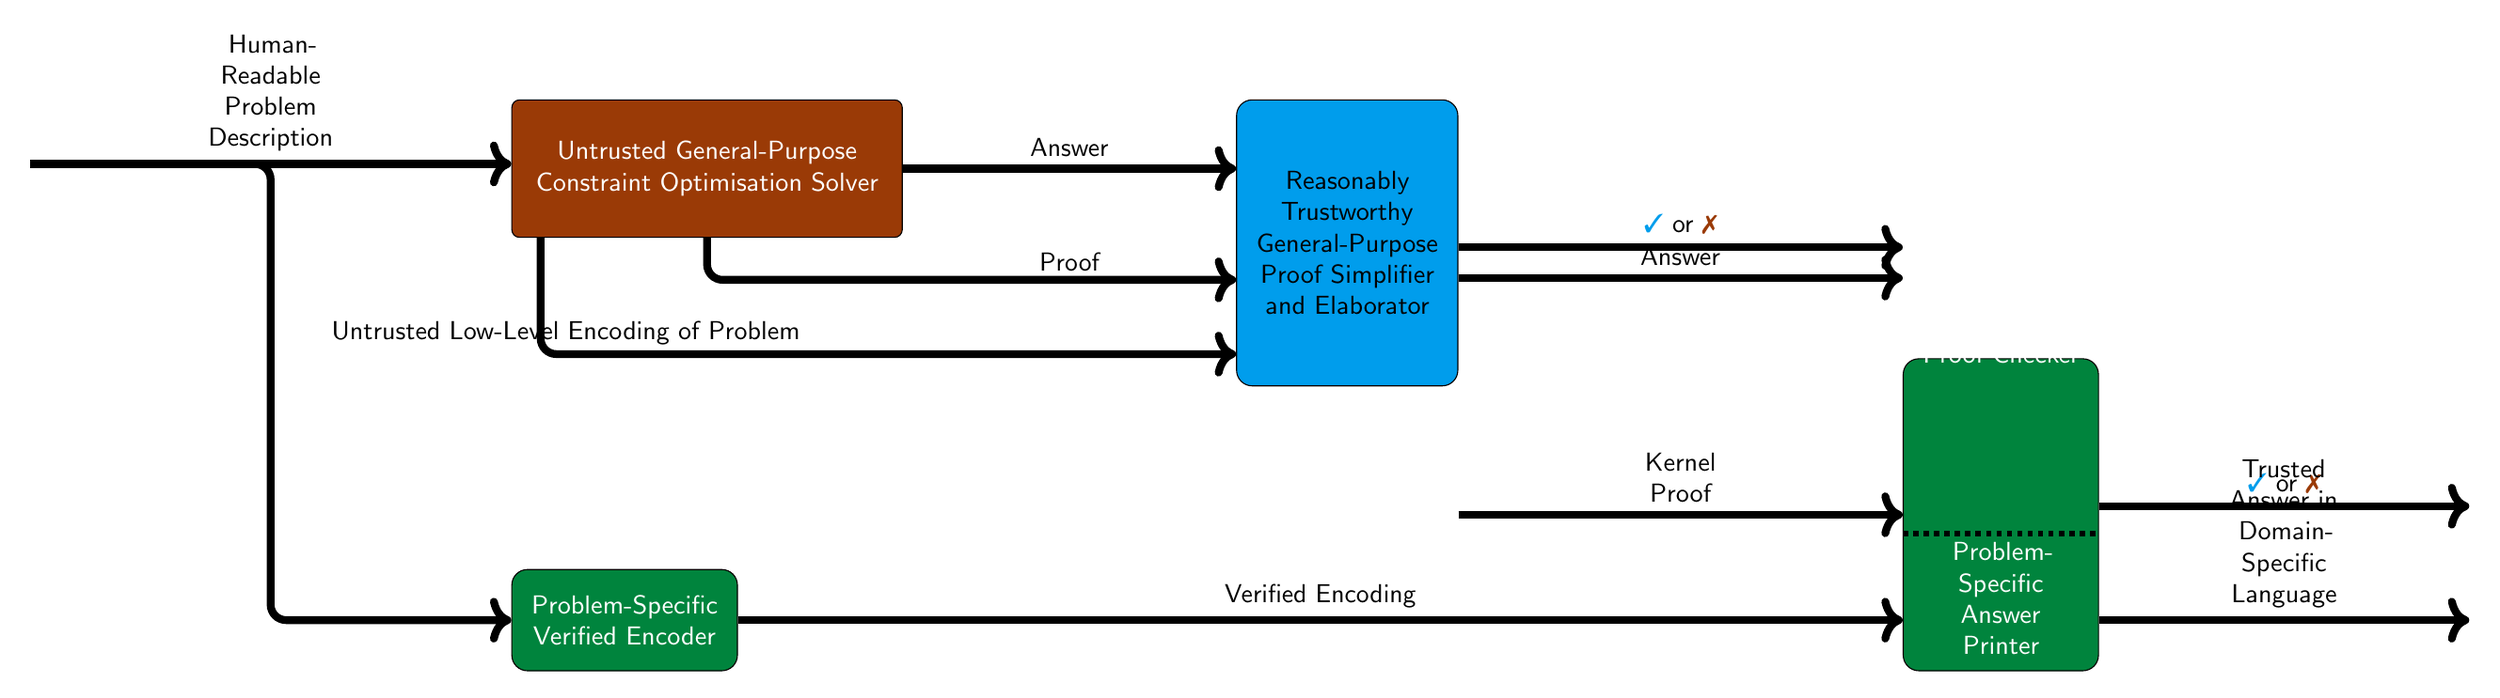
\begin{tikzpicture}
        \node (solver) [text centered, text width=14em, inner xsep=0.5em, inner ysep=1.6em, draw, rounded
        corners=3pt, fill=uofgrust, text=white] { Untrusted General-Purpose Constraint Optimisation Solver};

        \node (elaborator) [ right=4.5cm of solver.north east, anchor=north west, inner
        xsep=0.25em, draw, rounded corners=6pt, minimum height=11em, text width=8em, text centered,
        fill=uofgcobalt]
        { Reasonably Trustworthy General-Purpose Proof Simplifier and Elaborator };

        \node (verifiedchecker) [ right=6cm of elaborator.north east, anchor=north west, inner
            xsep=0.25em, draw, rounded corners=6pt, minimum height=12em, text width=7em, text
            centered, yshift=-3.5cm, fill=uofgleaf, text=white] { \phantom{Verified General-Purpose Proof Checker} };
        \node (gpverifiedchecker) [yshift=2.8cm, text width=6em, text centered, text=white] at (verifiedchecker)
            {Verified General-Purpose Proof Checker};
        \node (resultoutput) [anchor=south, yshift=0.3em, text width=4em, text centered, text=white] at (verifiedchecker.south)
            {Problem-Specific Answer Printer};

        \node (verifiedencoder) [ draw, rounded corners=6pt, text centered, anchor=south west,
        text width=8em, inner ysep=1em, fill=uofgleaf, text=white] at (solver.west|-verifiedchecker.south) {
            Problem-Specific Verified Encoder };

        \draw [->, line width=3pt] (solver.east) -- (solver.east -| elaborator.west)
            coordinate [midway] (solutionmid) node [above, midway] { Answer };

        \coordinate (elaboratorproofin) at ($(elaborator.west)+(0,-0.5)$);

        \draw [->, line width=3pt, rounded corners=6pt] (solver.south) -- (solver.south |- elaboratorproofin)
            -- (elaboratorproofin) coordinate [midway] (proofmid);

        \coordinate (prooflabel) at (proofmid-|solutionmid);
        \node [above=0cm of prooflabel] { Proof };

        \coordinate (verified) at ($(verifiedchecker.east)+($(5cm,3cm)$)$);
        \draw [->, line width=3pt] ($(verifiedchecker.north east)+(0cm,-2cm)$) -- ++(5cm,0cm)
            node [above, midway] { \textcolor{uofgcobalt}{\ding{51}} or \textcolor{uofgrust}{\ding{55}} };

        \coordinate (verifiedcheckertopleft) at ($(verifiedchecker.west)+($(0cm,3.2cm)$)$);
        \draw [->, line width=3pt] (elaborator.east |- verifiedcheckertopleft) --
        (verifiedcheckertopleft) node [above, midway, text width=4em, text centered] { Answer };
        \draw [->, line width=3pt] (elaborator.east |- verifiedchecker.west) -- (verifiedchecker.west) node [above, midway, text width=3em, text centered] { Kernel Proof };

        \coordinate (elaboratortopright) at ($(elaborator.north east)+(0.0,-2.0)$);
        \draw [->, line width=3pt] (elaboratortopright) -- (elaboratortopright-|verifiedchecker.west)
            node [above, midway] { \textcolor{uofgcobalt}{\ding{51}} or \textcolor{uofgrust}{\ding{55}} };

        \coordinate [above=1.0cm of solver.south west] (solverinputin);
        \coordinate [left=6.5cm of solverinputin] (input);
        \draw [->, line width=3pt] (input) -- (solverinputin) coordinate [midway] (inputmid) node [above,
        midway, text width=6em, text centered] { Human-Readable Problem Description };

        \coordinate (checkerbotleft) at
        ($(elaborator.west)+($(elaborator.west)-(solver.east-|elaborator.west)+(0,-0.5)$)$);

        \coordinate (solverstart) at ($(solver.south)!0.85!(solver.south west)$);
        \coordinate (solverstart2) at ($(solver.south)!0.75!(solver.south west)$);
        \draw [->, line width=3pt, rounded corners=6pt] (solverstart) -- (solverstart |- checkerbotleft) -- (checkerbotleft)
        coordinate [midway] (altinputmid);

        \coordinate (encinputlabel) at (altinputmid-|solutionmid);
        \node [above=0cm of encinputlabel, xshift=-6.8cm, text width=18em, text centered] { Untrusted
        Low-Level Encoding of Problem };

        \draw [->, line width=3pt, rounded corners=6pt] ($(inputmid)+(-0.2,0)$) -- (inputmid) -- (inputmid |-
        verifiedencoder.west) -- (verifiedencoder.west);

        \draw [->, line width=3pt] (verifiedencoder.east) -- (verifiedchecker.west|-verifiedencoder.east)
        node [above, midway] { Verified Encoding };

        \draw [->, line width=3pt] (verifiedchecker.east|-verifiedencoder.west) -- (verified|-verifiedencoder.west)
            node (trustedresult) [above, midway, text centered, text width=4.5em] { Trusted Answer in
            Domain-Specific Language };

        \draw [dotted, line width=2pt]
        (verifiedchecker.west|-resultoutput.north)--(verifiedchecker.east|-resultoutput.north);

    \end{tikzpicture}\end{center}

    \smallskip

    \textcolor{uofgleaf}{Formally verified programs} have extremely strong guarantees
    of correctness, but are expensive to implement and are limited in performance and functionality.
    A more complex toolchain lets us obtain formally verified answers from efficient solvers.
}


\begin{columns}
\column{0.52}

\block{Why is this Hard?}{
    Proofs need to be expressive and compositional, to efficiently capture all the reasoning carried
    out by intelligent combinatorial optimisation algorithms. But proof steps must also be simple,
    so we can trust and formally verify the proof system and checker.
    \vspace*{0.5cm}
}

\column{0.32}

\block{Further Reading}{
    \scriptsize
SG, CM, MOM, JN, AO, YKT: End-to-End Verification for Subgraph Solving. AAAI 2024.

\smallskip

BB, SG, CM, JN:
Certified Dominance and Symmetry Breaking for Combinatorial Optimisation. J. Artif. Intell. Res. 77. (2023)

\smallskip

MJM, CM:
Proof Logging for Smart Extensional Constraints. CP 2023.

\smallskip

SG: Certifying Correctness for Combinatorial Algorithms: by Using Pseudo-Boolean Reasoning. Lund
University, 2022. PhD Thesis.

\smallskip

SG, CM, JN:
An Auditable Constraint Programming Solver. CP 2022.
}

\column{0.16}

\block[]{Tutorial}{
    \vspace*{0.5cm}
    \begin{center}
    \qrcode[height=4cm]{https://bartbogaerts.eu/talks/veripb-tutorial-series/}
    \end{center}
    \vspace*{0.5cm}
}

\end{columns}


\begin{columns}
    \colorlet{blockbodybgcolor}{uofgsandstone!40!white}
    \colorlet{blocktitlebgcolor}{uofgsandstone!40!white}

    \column{0.84}

    \block[bodyinnersep=0mm, bodyverticalshift=-1mm]{}{\small
On two occasions I have been asked, -- ``Pray, Mr. Babbage, if you put into the machine wrong
figures, will the right answers come out?'' I am not able rightly to apprehend the kind of confusion
of ideas that could provoke such a question.
        }

    \column{0.16}
    \block[bodyinnersep=0mm, bodyverticalshift=-6mm]{}{\tiny
        Supported by a Royal Academy of Engineering Research Fellowship, and by the Engineering and Physical Sciences Research Council [grant number
        EP/X030032/1].
    }
\end{columns}

\end{document}

